\chapter{Scoping and Mindset}
	\label{ch:ScopingMindset}
		No matter how good one gets at the technical aspects of hacking, they will never be good at it if they do not understand how to think about their target and attack. 
		One must understand the difference between attempting to beat down a stone wall with a battering ram and simply finding the key. 
		In a world where the tools to run an attack are easy and often have a GUI with a big red ``hack the target'' button, such as Armitage's ``hail Mary'' feature, 
		we often forget to work out what our client is. 
		This section will have you step back, away from the keyboard and look at what is happening. 
		We will start with lock picking, as it is \emph{the} past time of hackers. 
		Then, we will move to researching the system that you are targeting. 
		However, this latter section will also require you to understand the information gathering tools explained in chapter \ref{ch:NetworkPenetration}.
	\section{Lock Picking}
		Before starting this section, you will need to either purchase or borrow a pick set and a clear or open cut lock. 
		A simple hook pick and tension wrench will suffice and if you cannot find a clear lock, a cheap padlock will be easy enough to practice on. 
		In this section, we will focus on the pin tumbler lock, which is the most common lock type used in cheap locking mechanisms, and the easiest to learn to pick. 
		An example of this type of lock can be seen in figure \ref{fig:PinTumblerLock}.\footnote{\url{https://commons.wikimedia.org/wiki/File:Pin\_and\_tumbler\_lock\_picking.PNG}}
		Furthermore, the ideas used in this section will be added to in later chapters, notably in chapter \ref{ch:WirelessAttacks} where we will clone NFC access cards. 
		\begin{figure}[htb]
			\centering
			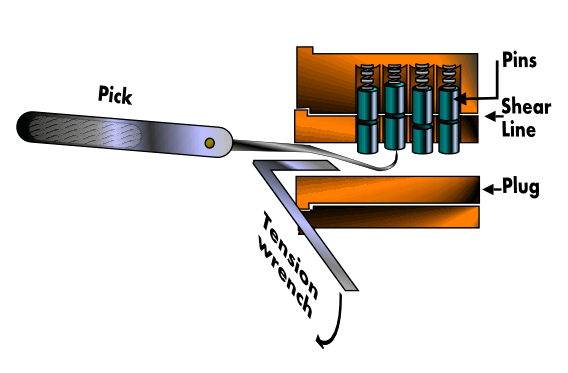
\includegraphics[scale=0.6]{./PinTumblerLock.png}
			\caption{Example of Picking a Pin and Tumbler Lock}
			\label{fig:PinTumblerLock}
		\end{figure}
		\subsection{How the Pin and Tumbler Lock Works}
			As can be seen in figure \ref{fig:PinTumblerLock}, this type of lock uses a number of sprint loaded pins which stop the plug of the lock moving within the housing. 
			Within this plug is a long, thin slot for the key (or our picks) with small ledges in the sides to both stop pins from falling and hinder those attempting to pick the lock. 
			A series of holes are drilled through the top of the housing and into the plug. 
			These holes are where the spring loaded pins enter, with the lower pin fully entering the plug and the upper pin being split across the sheer point. 
			It is this action which both allows the lock to remain closed when the key is not inserted and allows us to pick the lock. 
			When a torque is placed on the plug, some of these pins will begin to bind with the sheer point. 
			Using this, we can begin to pick the lock. 

		\subsection{Pin by Pin Picking}
			The first step when attempting to pick a lock is to place the tension wrench into the bottom of the lock and apply a slight pressure. 
			This pressure is designed to cause the top pins to catch on the sheer point of the plug, allowing some of the pins to bind. 
			Once this has occurred, a pick should be used to test each of the pins, determining how many there are and which ones have become bound to the sheer point. 

			The idea here is to place a small amount of pressure on the pins which bind to the sheer point in order of their binding. 
			This should leave the upper pin lodged above the plug, with the lower pin dropped into the key way. 
			Continue with this until either you have bound all pins and the lock is open, or you cannot determine whether pins have set or not. 
			If the latter, reset the pins by releasing pressure on the tension wrench. 
		\subsection{Raking}
			If on the other hand, you are the kind of person with little patience and a strong desire to get in, you can attempt raking. 
			In this process, you set the lock up in the same manner, but rather than attempting to find and set binding pins, you simply saw along the line. 
			When attempting this, no more than two pins are likely to set on each pass, with passes that set no pins being common. 
			Thus, you should repeatedly attempt rake until either the lock opens or you feel that you are getting no where. 
			During this process, you may also want to slightly adjust the amount of torque placed on the plug, however, be wary not to place too much torque on it. 

	\section{Research}
	\section{Problem Solving}
